\documentclass[conference]{IEEEtran}
\usepackage{graphicx,booktabs,xcolor,amsmath,cite,url}
\def\UrlBreaks{\do\/\do\-\do\.\do\_}
\graphicspath{{../results/}}
\newcommand{\todo}[1]{{\color{red}\textbf{[#1]}}}
% GENERATED by experiments/make_macros.py -- do not edit. Source of each macro in its trailing comment.
\newcommand{\ThreshCone}{10}% docs/SPEC.md C1 (spec constant)
\newcommand{\ThreshConeB}{100}% docs/SPEC.md C1b (spec constant)
\newcommand{\ThreshFourA}{20}% docs/SPEC.md C4a pct (spec constant)
\newcommand{\ThreshFourB}{10}% docs/SPEC.md C4b pct (spec constant)
\newcommand{\BudgetLut}{6,000}% docs/SPEC.md C3 (spec constant)
\newcommand{\BudgetMult}{40}% docs/SPEC.md C3 (spec constant)
\newcommand{\BudgetBram}{12}% docs/SPEC.md C3 (spec constant)
\newcommand{\RandomLayers}{1,000}% docs/SPEC.md C2a (spec constant)
\newcommand{\ImagesCtwoB}{10}% docs/SPEC.md C2b (spec constant)
\newcommand{\ImagesCtwoC}{100}% docs/SPEC.md C2c (spec constant)
\newcommand{\PDefault}{8}% docs/SPEC.md default P (spec constant)
\newcommand{\PMax}{16}% docs/SPEC.md P sweep (spec constant)
\newcommand{\Lanes}{4}% docs/SPEC.md DESIGN 5 lanes per output channel (spec constant)
\newcommand{\DescWords}{18}% docs/SPEC.md DESIGN 6.2 descriptor words (spec constant)
\newcommand{\WbufRows}{512}% docs/SPEC.md section 7 weight buffer rows (spec constant)
\newcommand{\PortBits}{32}% docs/SPEC.md section 2 accelerator RAM port width (spec constant)
\newcommand{\RamMiB}{1}% docs/SPEC.md section 7 simulated RAM (spec constant)
\newcommand{\Pvone}{1}% docs/SPEC.md section 2 (P grid value, table row label)
\newcommand{\Pvtwo}{2}% docs/SPEC.md section 2 (P grid value, table row label)
\newcommand{\Pvfour}{4}% docs/SPEC.md section 2 (P grid value, table row label)
\newcommand{\Pveight}{8}% docs/SPEC.md section 2 (P grid value, table row label)
\newcommand{\Pvsixteen}{16}% docs/SPEC.md section 2 (P grid value, table row label)
\newcommand{\PGrid}{1, 2, 4, 8, 16}% docs/SPEC.md section 2 (P ablation grid)
\newcommand{\MOneCommit}{6533b1e9f9f2b7c46bb8dbca5d205ab71fca11ff}% git rev-parse m1^{}
\newcommand{\MOneCommitShort}{6533b1e}% git rev-parse m1^{}
\newcommand{\MOneCsvSha}{fd94f39a1a913ee63cb03e4a9cd256cc42e6ca0df9dd0c5383c50ac62e4bd362}% sha256 of results/m1_predictions.csv at tag m1
\newcommand{\MOneCsvShaShort}{fd94f39a1a913ee6}% sha256 of results/m1_predictions.csv at tag m1
\newcommand{\MOneModelCommit}{1f4fa47}% results/m1_summary.json commit
\newcommand{\MOneRowsAll}{324}% data rows of results/m1_predictions.csv (all archs)
\newcommand{\MOneRows}{108}% rows with arch=os in results/m1_predictions.csv
\newcommand{\MOneRowsPone}{32}% rows with arch=os and P=1
\newcommand{\MOneRowsPtwo}{23}% rows with arch=os and P=2
\newcommand{\MOneRowsPfour}{19}% rows with arch=os and P=4
\newcommand{\MOneRowsPeight}{17}% rows with arch=os and P=8
\newcommand{\MOneRowsPsixteen}{17}% rows with arch=os and P=16
\newcommand{\BenchWindow}{120}% results/baseline_overhead.json cycles_median
\newcommand{\DrvChain}{71}% results/driver_overhead.json drv_chain
\newcommand{\DrvPatch}{15}% results/driver_overhead.json drv_patch
\newcommand{\BaselineCyclesMnist}{12,188,028}% results/baseline_mnist_cnn.json mcugrad_result.cycles_median
\newcommand{\BaselineMinMnist}{12,183,011}% results/baseline_mnist_cnn.json mcugrad_result.cycles_min
\newcommand{\BaselineMaxMnist}{12,193,076}% results/baseline_mnist_cnn.json mcugrad_result.cycles_max
\newcommand{\BaselineMsMnist}{243.8}% results/baseline_mnist_cnn.json cycles_median / clock_hz
\newcommand{\BaselineImagesMnist}{10}% results/baseline_mnist_cnn.json images
\newcommand{\BaselineRunsMnist}{3}% results/baseline_mnist_cnn.json runs
\newcommand{\BaselineCorrectMnist}{10}% results/baseline_mnist_cnn.json mcugrad_result.correct (of images)
\newcommand{\ClockMHzMnist}{50}% results/baseline_mnist_cnn.json clock_hz
\newcommand{\ProfileAccelShareMnist}{96.4}% sum of ops[].share with name conv2d*/matmul* in baseline_profile_mnist_cnn.json (pct)
\newcommand{\ProfileSwShareMnist}{3.6}% sum of ops[].share, pool/transpose ops, baseline_profile_mnist_cnn.json (pct)
\newcommand{\BaselineCyclesCifar}{72,157,425}% results/baseline_cifar_mobilenet.json mcugrad_result.cycles_median
\newcommand{\BaselineMinCifar}{72,132,576}% results/baseline_cifar_mobilenet.json mcugrad_result.cycles_min
\newcommand{\BaselineMaxCifar}{72,174,963}% results/baseline_cifar_mobilenet.json mcugrad_result.cycles_max
\newcommand{\BaselineMsCifar}{1443.1}% results/baseline_cifar_mobilenet.json cycles_median / clock_hz
\newcommand{\BaselineImagesCifar}{10}% results/baseline_cifar_mobilenet.json images
\newcommand{\BaselineRunsCifar}{3}% results/baseline_cifar_mobilenet.json runs
\newcommand{\BaselineCorrectCifar}{8}% results/baseline_cifar_mobilenet.json mcugrad_result.correct (of images)
\newcommand{\ClockMHzCifar}{50}% results/baseline_cifar_mobilenet.json clock_hz
\newcommand{\ProfileAccelShareCifar}{99.9}% sum of ops[].share with name conv2d*/matmul* in baseline_profile_cifar_mobilenet.json (pct)
\newcommand{\ProfileSwShareCifar}{0.1}% sum of ops[].share, pool/transpose ops, baseline_profile_cifar_mobilenet.json (pct)
\newcommand{\PredSpeedupMnistPone}{22.9}% m1_summary.json models.mnist_cnn.archs.os.P.1.predicted_speedup
\newcommand{\PredStampMnistPone}{98,312}% m1_summary.json models.mnist_cnn.archs.os.P.1.sum_stamp
\newcommand{\PredModelRunMnistPone}{531,982}% m1_summary.json models.mnist_cnn.archs.os.P.1.predicted_model_run
\newcommand{\PredSpeedupMnistPtwo}{25.2}% m1_summary.json models.mnist_cnn.archs.os.P.2.predicted_speedup
\newcommand{\PredStampMnistPtwo}{50,888}% m1_summary.json models.mnist_cnn.archs.os.P.2.sum_stamp
\newcommand{\PredModelRunMnistPtwo}{484,524}% m1_summary.json models.mnist_cnn.archs.os.P.2.predicted_model_run
\newcommand{\PredSpeedupMnistPfour}{26.4}% m1_summary.json models.mnist_cnn.archs.os.P.4.predicted_speedup
\newcommand{\PredStampMnistPfour}{27,697}% m1_summary.json models.mnist_cnn.archs.os.P.4.sum_stamp
\newcommand{\PredModelRunMnistPfour}{461,316}% m1_summary.json models.mnist_cnn.archs.os.P.4.predicted_model_run
\newcommand{\PredSpeedupMnistPeight}{27.0}% m1_summary.json models.mnist_cnn.archs.os.P.8.predicted_speedup
\newcommand{\PredStampMnistPeight}{18,496}% m1_summary.json models.mnist_cnn.archs.os.P.8.sum_stamp
\newcommand{\PredModelRunMnistPeight}{452,098}% m1_summary.json models.mnist_cnn.archs.os.P.8.predicted_model_run
\newcommand{\PredSpeedupMnistPsixteen}{27.2}% m1_summary.json models.mnist_cnn.archs.os.P.16.predicted_speedup
\newcommand{\PredStampMnistPsixteen}{15,156}% m1_summary.json models.mnist_cnn.archs.os.P.16.sum_stamp
\newcommand{\PredModelRunMnistPsixteen}{448,758}% m1_summary.json models.mnist_cnn.archs.os.P.16.predicted_model_run
\newcommand{\PredAccelChainsMnistPeight}{18,508}% m1_summary.json models.mnist_cnn.archs.os.P.8.accel_cycles
\newcommand{\PredSwCyclesMnistPeight}{433,242}% m1_summary.json models.mnist_cnn.archs.os.P.8.sw_cycles
\newcommand{\PredDriverMnistPeight}{228}% m1_summary.json models.mnist_cnn.archs.os.P.8.driver_cycles
\newcommand{\PredCfourBMnistPeight}{18,736}% m1_summary.json models.mnist_cnn.archs.os.P.8.c4b_pred_cycles
\newcommand{\PredCommandsMnistPeight}{3}% m1_summary.json models.mnist_cnn.archs.os.P.8.n_commands
\newcommand{\PredChainsMnistPeight}{3}% m1_summary.json models.mnist_cnn.archs.os.P.8.n_chains
\newcommand{\PredUtilMnistPeight}{56.1}% m1_summary.json models.mnist_cnn.archs.os.P.8.util (pct)
\newcommand{\PredSwShareMnistPeight}{95.8}% m1_summary.json models.mnist_cnn.archs.os.P.8.sw_cycles / predicted_model_run (pct)
\newcommand{\PredPstarMnist}{16}% m1_summary.json models.mnist_cnn.archs.os.p_star (16 = not reached)
\newcommand{\PredPstarEndMnist}{2}% m1_summary.json models.mnist_cnn.archs.os.p_star_end_to_end
\newcommand{\PredSpeedupCifarPone}{111.7}% m1_summary.json models.cifar_mobilenet.archs.os.P.1.predicted_speedup
\newcommand{\PredStampCifarPone}{582,676}% m1_summary.json models.cifar_mobilenet.archs.os.P.1.sum_stamp
\newcommand{\PredModelRunCifarPone}{645,778}% m1_summary.json models.cifar_mobilenet.archs.os.P.1.predicted_model_run
\newcommand{\PredSpeedupCifarPtwo}{187.1}% m1_summary.json models.cifar_mobilenet.archs.os.P.2.predicted_speedup
\newcommand{\PredStampCifarPtwo}{322,660}% m1_summary.json models.cifar_mobilenet.archs.os.P.2.sum_stamp
\newcommand{\PredModelRunCifarPtwo}{385,748}% m1_summary.json models.cifar_mobilenet.archs.os.P.2.predicted_model_run
\newcommand{\PredSpeedupCifarPfour}{282.0}% m1_summary.json models.cifar_mobilenet.archs.os.P.4.predicted_speedup
\newcommand{\PredStampCifarPfour}{192,788}% m1_summary.json models.cifar_mobilenet.archs.os.P.4.sum_stamp
\newcommand{\PredModelRunCifarPfour}{255,870}% m1_summary.json models.cifar_mobilenet.archs.os.P.4.predicted_model_run
\newcommand{\PredSpeedupCifarPeight}{363.1}% m1_summary.json models.cifar_mobilenet.archs.os.P.8.predicted_speedup
\newcommand{\PredStampCifarPeight}{135,672}% m1_summary.json models.cifar_mobilenet.archs.os.P.8.sum_stamp
\newcommand{\PredModelRunCifarPeight}{198,752}% m1_summary.json models.cifar_mobilenet.archs.os.P.8.predicted_model_run
\newcommand{\PredSpeedupCifarPsixteen}{411.4}% m1_summary.json models.cifar_mobilenet.archs.os.P.16.predicted_speedup
\newcommand{\PredStampCifarPsixteen}{112,308}% m1_summary.json models.cifar_mobilenet.archs.os.P.16.sum_stamp
\newcommand{\PredModelRunCifarPsixteen}{175,388}% m1_summary.json models.cifar_mobilenet.archs.os.P.16.predicted_model_run
\newcommand{\PredAccelChainsCifarPeight}{135,704}% m1_summary.json models.cifar_mobilenet.archs.os.P.8.accel_cycles
\newcommand{\PredSwCyclesCifarPeight}{62,756}% m1_summary.json models.cifar_mobilenet.archs.os.P.8.sw_cycles
\newcommand{\PredDriverCifarPeight}{172}% m1_summary.json models.cifar_mobilenet.archs.os.P.8.driver_cycles
\newcommand{\PredCfourBCifarPeight}{135,876}% m1_summary.json models.cifar_mobilenet.archs.os.P.8.c4b_pred_cycles
\newcommand{\PredCommandsCifarPeight}{14}% m1_summary.json models.cifar_mobilenet.archs.os.P.8.n_commands
\newcommand{\PredChainsCifarPeight}{2}% m1_summary.json models.cifar_mobilenet.archs.os.P.8.n_chains
\newcommand{\PredUtilCifarPeight}{45.0}% m1_summary.json models.cifar_mobilenet.archs.os.P.8.util (pct)
\newcommand{\PredSwShareCifarPeight}{31.6}% m1_summary.json models.cifar_mobilenet.archs.os.P.8.sw_cycles / predicted_model_run (pct)
\newcommand{\PredPstarCifar}{16}% m1_summary.json models.cifar_mobilenet.archs.os.p_star (16 = not reached)
\newcommand{\PredPstarEndCifar}{16}% m1_summary.json models.cifar_mobilenet.archs.os.p_star_end_to_end
\newcommand{\MeasCyclesMnistPone}{\todo{MEASURE: accelerated cycles mnist cnn P=1}}% PENDING results/m5_accel_mnist_cnn_P1.json
\newcommand{\MeasSpeedupMnistPone}{\todo{MEASURE: speedup mnist cnn P=1}}% PENDING results/m5_accel_mnist_cnn_P1.json
\newcommand{\MeasCyclesMnistPtwo}{\todo{MEASURE: accelerated cycles mnist cnn P=2}}% PENDING results/m5_accel_mnist_cnn_P2.json
\newcommand{\MeasSpeedupMnistPtwo}{\todo{MEASURE: speedup mnist cnn P=2}}% PENDING results/m5_accel_mnist_cnn_P2.json
\newcommand{\MeasCyclesMnistPfour}{\todo{MEASURE: accelerated cycles mnist cnn P=4}}% PENDING results/m5_accel_mnist_cnn_P4.json
\newcommand{\MeasSpeedupMnistPfour}{\todo{MEASURE: speedup mnist cnn P=4}}% PENDING results/m5_accel_mnist_cnn_P4.json
\newcommand{\MeasCyclesMnistPeight}{\todo{MEASURE: accelerated cycles mnist cnn P=8}}% PENDING results/m5_accel_mnist_cnn_P8.json
\newcommand{\MeasSpeedupMnistPeight}{\todo{MEASURE: speedup mnist cnn P=8}}% PENDING results/m5_accel_mnist_cnn_P8.json
\newcommand{\MeasCyclesMnistPsixteen}{\todo{MEASURE: accelerated cycles mnist cnn P=16}}% PENDING results/m5_accel_mnist_cnn_P16.json
\newcommand{\MeasSpeedupMnistPsixteen}{\todo{MEASURE: speedup mnist cnn P=16}}% PENDING results/m5_accel_mnist_cnn_P16.json
\newcommand{\MeasCyclesCifarPone}{\todo{MEASURE: accelerated cycles cifar mobilenet P=1}}% PENDING results/m5_accel_cifar_mobilenet_P1.json
\newcommand{\MeasSpeedupCifarPone}{\todo{MEASURE: speedup cifar mobilenet P=1}}% PENDING results/m5_accel_cifar_mobilenet_P1.json
\newcommand{\MeasCyclesCifarPtwo}{\todo{MEASURE: accelerated cycles cifar mobilenet P=2}}% PENDING results/m5_accel_cifar_mobilenet_P2.json
\newcommand{\MeasSpeedupCifarPtwo}{\todo{MEASURE: speedup cifar mobilenet P=2}}% PENDING results/m5_accel_cifar_mobilenet_P2.json
\newcommand{\MeasCyclesCifarPfour}{\todo{MEASURE: accelerated cycles cifar mobilenet P=4}}% PENDING results/m5_accel_cifar_mobilenet_P4.json
\newcommand{\MeasSpeedupCifarPfour}{\todo{MEASURE: speedup cifar mobilenet P=4}}% PENDING results/m5_accel_cifar_mobilenet_P4.json
\newcommand{\MeasCyclesCifarPeight}{\todo{MEASURE: accelerated cycles cifar mobilenet P=8}}% PENDING results/m5_accel_cifar_mobilenet_P8.json
\newcommand{\MeasSpeedupCifarPeight}{\todo{MEASURE: speedup cifar mobilenet P=8}}% PENDING results/m5_accel_cifar_mobilenet_P8.json
\newcommand{\MeasCyclesCifarPsixteen}{\todo{MEASURE: accelerated cycles cifar mobilenet P=16}}% PENDING results/m5_accel_cifar_mobilenet_P16.json
\newcommand{\MeasSpeedupCifarPsixteen}{\todo{MEASURE: speedup cifar mobilenet P=16}}% PENDING results/m5_accel_cifar_mobilenet_P16.json
\newcommand{\VerdictCone}{\todo{MEASURE: C1 verdict}}% PENDING C1 from m5_accel_*_P8.json
\newcommand{\VerdictConeB}{\todo{MEASURE: C1b verdict}}% PENDING C1b from m5_accel_cifar_mobilenet_P8.json
\newcommand{\MeasCtwoALayers}{\todo{MEASURE: C2a layers run}}% PENDING results/m3_bitexact.csv
\newcommand{\MeasCtwoAMismatch}{\todo{MEASURE: C2a mismatching bytes}}% PENDING results/m3_bitexact.csv
\newcommand{\VerdictCtwoA}{\todo{MEASURE: C2a verdict}}% PENDING results/m3_bitexact.csv
\newcommand{\MeasCtwoBImages}{\todo{MEASURE: c2b images}}% PENDING results/m5_bitexact.json
\newcommand{\MeasCtwoBMismatch}{\todo{MEASURE: c2b mismatch}}% PENDING results/m5_bitexact.json
\newcommand{\MeasCtwoCImages}{\todo{MEASURE: c2c images}}% PENDING results/m5_bitexact.json
\newcommand{\MeasCtwoCMismatch}{\todo{MEASURE: c2c mismatch}}% PENDING results/m5_bitexact.json
\newcommand{\SynPicorvLut}{2,896}% results/syn/picorv32.jsonl seed 1 .lut4
\newcommand{\SynPicorvFf}{1,027}% results/syn/picorv32.jsonl seed 1 .ff
\newcommand{\SynPicorvBram}{0}% results/syn/picorv32.jsonl seed 1 .dp16kd
\newcommand{\SynPicorvMult}{4}% results/syn/picorv32.jsonl seed 1 .mult18x18d
\newcommand{\SynPicorvFmax}{78.2}% results/syn/picorv32.jsonl median fmax_mhz over 1 seeds
\newcommand{\SynPicorvFmaxSeeds}{1}% results/syn/picorv32.jsonl seeds
\newcommand{\SynSocNoAccelLut}{3,224}% results/syn/soc_noaccel.jsonl seed 1 .lut4
\newcommand{\SynSocNoAccelFf}{1,073}% results/syn/soc_noaccel.jsonl seed 1 .ff
\newcommand{\SynSocNoAccelBram}{128}% results/syn/soc_noaccel.jsonl seed 1 .dp16kd
\newcommand{\SynSocNoAccelMult}{4}% results/syn/soc_noaccel.jsonl seed 1 .mult18x18d
\newcommand{\SynSocNoAccelFmax}{63.1}% results/syn/soc_noaccel.jsonl median fmax_mhz over 1 seeds
\newcommand{\SynSocNoAccelFmaxSeeds}{1}% results/syn/soc_noaccel.jsonl seeds
\newcommand{\SynSocPeightLut}{\todo{MEASURE: soc lut4}}% PENDING results/syn/soc_P8.jsonl
\newcommand{\SynSocPeightFf}{\todo{MEASURE: soc ff}}% PENDING results/syn/soc_P8.jsonl
\newcommand{\SynSocPeightBram}{\todo{MEASURE: soc dp16kd}}% PENDING results/syn/soc_P8.jsonl
\newcommand{\SynSocPeightMult}{\todo{MEASURE: soc mult18x18d}}% PENDING results/syn/soc_P8.jsonl
\newcommand{\SynSocPeightFmax}{\todo{MEASURE: soc Fmax}}% PENDING results/syn/soc_P8.jsonl
\newcommand{\SynSocPeightFmaxSeeds}{\todo{MEASURE: soc seeds}}% PENDING results/syn/soc_P8.jsonl
\newcommand{\SynAccelPoneLut}{\todo{MEASURE: accel lut4}}% PENDING results/syn/accel_P1.jsonl
\newcommand{\SynAccelPoneFf}{\todo{MEASURE: accel ff}}% PENDING results/syn/accel_P1.jsonl
\newcommand{\SynAccelPoneBram}{\todo{MEASURE: accel dp16kd}}% PENDING results/syn/accel_P1.jsonl
\newcommand{\SynAccelPoneMult}{\todo{MEASURE: accel mult18x18d}}% PENDING results/syn/accel_P1.jsonl
\newcommand{\SynAccelPoneFmax}{\todo{MEASURE: accel Fmax}}% PENDING results/syn/accel_P1.jsonl
\newcommand{\SynAccelPoneFmaxSeeds}{\todo{MEASURE: accel seeds}}% PENDING results/syn/accel_P1.jsonl
\newcommand{\SynAccelPtwoLut}{\todo{MEASURE: accel lut4}}% PENDING results/syn/accel_P2.jsonl
\newcommand{\SynAccelPtwoFf}{\todo{MEASURE: accel ff}}% PENDING results/syn/accel_P2.jsonl
\newcommand{\SynAccelPtwoBram}{\todo{MEASURE: accel dp16kd}}% PENDING results/syn/accel_P2.jsonl
\newcommand{\SynAccelPtwoMult}{\todo{MEASURE: accel mult18x18d}}% PENDING results/syn/accel_P2.jsonl
\newcommand{\SynAccelPtwoFmax}{\todo{MEASURE: accel Fmax}}% PENDING results/syn/accel_P2.jsonl
\newcommand{\SynAccelPtwoFmaxSeeds}{\todo{MEASURE: accel seeds}}% PENDING results/syn/accel_P2.jsonl
\newcommand{\SynAccelPfourLut}{\todo{MEASURE: accel lut4}}% PENDING results/syn/accel_P4.jsonl
\newcommand{\SynAccelPfourFf}{\todo{MEASURE: accel ff}}% PENDING results/syn/accel_P4.jsonl
\newcommand{\SynAccelPfourBram}{\todo{MEASURE: accel dp16kd}}% PENDING results/syn/accel_P4.jsonl
\newcommand{\SynAccelPfourMult}{\todo{MEASURE: accel mult18x18d}}% PENDING results/syn/accel_P4.jsonl
\newcommand{\SynAccelPfourFmax}{\todo{MEASURE: accel Fmax}}% PENDING results/syn/accel_P4.jsonl
\newcommand{\SynAccelPfourFmaxSeeds}{\todo{MEASURE: accel seeds}}% PENDING results/syn/accel_P4.jsonl
\newcommand{\SynAccelPeightLut}{\todo{MEASURE: accel lut4}}% PENDING results/syn/accel_P8.jsonl
\newcommand{\SynAccelPeightFf}{\todo{MEASURE: accel ff}}% PENDING results/syn/accel_P8.jsonl
\newcommand{\SynAccelPeightBram}{\todo{MEASURE: accel dp16kd}}% PENDING results/syn/accel_P8.jsonl
\newcommand{\SynAccelPeightMult}{\todo{MEASURE: accel mult18x18d}}% PENDING results/syn/accel_P8.jsonl
\newcommand{\SynAccelPeightFmax}{\todo{MEASURE: accel Fmax}}% PENDING results/syn/accel_P8.jsonl
\newcommand{\SynAccelPeightFmaxSeeds}{\todo{MEASURE: accel seeds}}% PENDING results/syn/accel_P8.jsonl
\newcommand{\SynAccelPsixteenLut}{\todo{MEASURE: accel lut4}}% PENDING results/syn/accel_P16.jsonl
\newcommand{\SynAccelPsixteenFf}{\todo{MEASURE: accel ff}}% PENDING results/syn/accel_P16.jsonl
\newcommand{\SynAccelPsixteenBram}{\todo{MEASURE: accel dp16kd}}% PENDING results/syn/accel_P16.jsonl
\newcommand{\SynAccelPsixteenMult}{\todo{MEASURE: accel mult18x18d}}% PENDING results/syn/accel_P16.jsonl
\newcommand{\SynAccelPsixteenFmax}{\todo{MEASURE: accel Fmax}}% PENDING results/syn/accel_P16.jsonl
\newcommand{\SynAccelPsixteenFmaxSeeds}{\todo{MEASURE: accel seeds}}% PENDING results/syn/accel_P16.jsonl
\newcommand{\VerdictCthree}{\todo{MEASURE: C3 verdict}}% PENDING C3 from syn/accel_P8.jsonl
\newcommand{\MeasCfourRows}{\todo{MEASURE: C4a rows}}% PENDING results/m6_pred_vs_meas.csv
\newcommand{\MeasCfourMaxErr}{\todo{MEASURE: C4a max error}}% PENDING results/m6_pred_vs_meas.csv
\newcommand{\MeasCfourMedianErr}{\todo{MEASURE: C4a median signed error}}% PENDING results/m6_pred_vs_meas.csv
\newcommand{\MeasCfourViolations}{\todo{MEASURE: C4a violations}}% PENDING results/m6_pred_vs_meas.csv
\newcommand{\VerdictCfourA}{\todo{MEASURE: C4a verdict}}% PENDING results/m6_pred_vs_meas.csv
\newcommand{\MeasCfourBMnist}{\todo{MEASURE: C4b measured mnist cnn}}% PENDING results/m6_c4b.json
\newcommand{\MeasCfourBErrMnist}{\todo{MEASURE: C4b error mnist cnn}}% PENDING results/m6_c4b.json
\newcommand{\MeasCfourBCifar}{\todo{MEASURE: C4b measured cifar mobilenet}}% PENDING results/m6_c4b.json
\newcommand{\MeasCfourBErrCifar}{\todo{MEASURE: C4b error cifar mobilenet}}% PENDING results/m6_c4b.json
\newcommand{\PstarMeasMnist}{\todo{MEASURE: measured saturation width}}% PENDING results/m5_accel_*_P*.json (sum STAMP)
\newcommand{\PstarMeasCifar}{\todo{MEASURE: measured saturation width}}% PENDING results/m5_accel_*_P*.json (sum STAMP)

\newcommand{\tabtodo}{\renewcommand{\todo}[1]{{\color{red}\textbf{?}}}}% compact pending marker inside tables
\newcommand{\sys}{\textsc{mcuaccel}}
\newcommand{\row}[1]{\csname Pv#1\endcsname & \csname PredSpeedupMnistP#1\endcsname & \csname MeasSpeedupMnistP#1\endcsname & \csname PredSpeedupCifarP#1\endcsname & \csname MeasSpeedupCifarP#1\endcsname\\}

\begin{document}
\title{A Pre-Registered Cost Model for a Small Bit-Exact int8 CNN Accelerator on a RISC-V Microcontroller SoC}
\author{\IEEEauthorblockN{Anonymous for review}}
\maketitle

\begin{abstract}
We present \sys{}, an int8 convolution, depthwise and fully connected accelerator memory-mapped into a PicoRV32 SoC, together with a backend for \texttt{mcugrad} that emits accelerator command descriptors and driver C while keeping every other operator in the original software kernels. The accelerator targets bit-exactness with the TFLite-style integer reference. Its cycle counts are predicted by an analytic port-bound model whose predictions were committed to git (tag \texttt{m1}, \MOneCommitShort) before any datapath RTL existed. At $P=\PDefault$ the frozen model predicts a speedup of \PredSpeedupMnistPeight$\times$ on \texttt{mnist\_cnn} and \PredSpeedupCifarPeight$\times$ on \texttt{cifar\_mobilenet}; these were computed against the software baselines measured before decision D19, an inlining fix after which the baselines are \BaselineCyclesMnist{} and \BaselineCyclesCifar{} cycles per inference. Measured against the current baselines: \MeasSpeedupMnistPeight$\times$ and \MeasSpeedupCifarPeight$\times$. A post-hoc rescoring, which substitutes the measured post-D19 fallback-operator cycles into the frozen accelerator-plus-driver prediction, gives \PostHocSpeedupMnist$\times$ and \PostHocSpeedupCifar$\times$. Claim C1 is \VerdictCone{}; C4a is \VerdictCfourA{}, although \NExceed{} commands exceeded their pre-registered bias (root cause given post hoc below); C3 is \VerdictCthree{}: \SynAccelPeightLut{} LUT4 against a budget of \BudgetLut. All cycle counts are Verilator cycles, not FPGA wall-clock.
\end{abstract}

\section{Introduction}
Quantized CNNs cost tens of millions of cycles per image on microcontroller-class cores. A dedicated int8 accelerator beating a scalar in-order RISC-V core by an order of magnitude or more is well established \cite{genc2021gemmini,prakash2023cfu,moreau2018vta}; reproducing that is not our contribution. We ask instead how well a simple analytic model, written down \emph{before} the RTL, predicts the cycle counts of a small memory-bound accelerator, with tolerances fixed in advance. The claims below are pre-registered in \texttt{docs/SPEC.md}; the predictions are frozen at tag \texttt{m1} (commit \texttt{\MOneCommitShort}, \texttt{m1\_predictions.csv} sha256 prefix \texttt{\MOneCsvShaShort}).

\begin{description}\setlength{\itemsep}{0pt}
\item[C1] Speedup at $P=\PDefault$ is at least \ThreshCone$\times$ on both networks, end to end with fallback layers and driver. \textbf{C1b}: at least \ThreshConeB$\times$ on \texttt{cifar\_mobilenet}.
\item[C2] Bit-exactness: zero mismatching bytes on \RandomLayers{} random layers (C2a), in every intermediate tensor of both networks (C2b), and in final outputs for \ImagesCtwoC{} images per network on the full SoC (C2c).
\item[C3] At $P=\PDefault$ the accelerator uses at most \BudgetLut{} LUT4, \BudgetMult{} \texttt{MULT18X18D} and \BudgetBram{} \texttt{DP16KD} on an ECP5 LFE5U-85F.
\item[C4] The frozen model predicts every accelerator command within \ThreshFourA\,\% (C4a, all $P$) and each network's accelerator-plus-driver time within \ThreshFourB\,\% (C4b).
\item[C5] The saturation width of the $P$ sweep is reported, predicted versus measured; its mechanism was stated in advance.
\end{description}

\section{Background and Related Work}
\textbf{Quantization.} The numerical contract is the integer-only scheme of Jacob et al.~\cite{jacob2018quantization} as implemented in gemmlowp~\cite{gemmlowp_fixedpoint} and specified by LiteRT~\cite{litert_quantspec}: a saturating rounding doubling high multiply followed by a rounding divide by a power of two. \textbf{MCU inference.} TFLite Micro~\cite{david2021tflm}, CMSIS-NN~\cite{lai2018cmsisnn} and MCUNet~\cite{lin2020mcunet} provide software kernels; \texttt{mcugrad}~\cite{mcugrad_repo} is the compiler whose int8 simulator is our specification.
\textbf{Accelerators.} Eyeriss~\cite{chen2016eyeriss}, the TPU~\cite{jouppi2017tpu}, NVDLA~\cite{nvdla_hw}, VTA~\cite{moreau2018vta}, Gemmini~\cite{genc2021gemmini} and CFU Playground~\cite{prakash2023cfu} show large speedups over in-order cores; FINN~\cite{umuroglu2017finn} and PULP-NN~\cite{garofalo2019pulpnn} target FPGA and multicore MCU settings. None of their RTL is used here. \textbf{Models.} Earlier analytic models~\cite{zhang2015optimizing,alwani2016fused} and the roofline model~\cite{williams2009roofline} were fitted alongside their designs; ours was frozen first. The CPU is PicoRV32~\cite{picorv32} on a Lattice ECP5~\cite{lattice_ecp5}, with the bus protocol of corv32~\cite{corv32_repo}.

\section{Architecture}
The CPU reaches a dual-port RAM through an adapter and interconnect; the accelerator is a second bus master on the RAM's other port (a private \PortBits-bit port, one word per cycle, one outstanding request), so no arbiter is needed. The CPU writes a descriptor address and a start bit, then polls a status register (Fig.~\ref{fig:sys}).

\begin{figure}[t]\centering\small
\fbox{\parbox{0.93\columnwidth}{\centering
PicoRV32 $\to$ adapter $\to$ interconnect $\to$ \{RAM port A, console, accelerator registers\}\\[2pt]
fetch (only master) $\to$ ctrl (descriptor FSM, loop nest) $\to$ align $\to$ MAC array ($P$ outputs $\times$ \Lanes{} lanes) $\to$ requant $\to$ writer $\to$ RAM port B}}
\caption{System block diagram (schematic; \texttt{docs/DESIGN.md} Sec.~1).}\label{fig:sys}
\end{figure}

\textbf{Dataflow.} The array is output-stationary over one output pixel and a tile of $P$ output channels. In NHWC layout the in-bounds part of a kernel row is contiguous, so each cycle one four-byte activation word meets one weight-buffer row of $\Lanes\cdot P$ bytes and performs $\Lanes\cdot P$ multiply-accumulates; every channel count uses one mechanism. Depthwise layers get only \Lanes{} useful MACs per cycle. Weights and per-channel parameters are loaded once per command into local buffers (\WbufRows{} rows). A single requantizer emits one byte per cycle using the specification's SRDHM/RDBPOT rule; accumulators are 32 bit and the backend enforces a no-wrap bound.

\textbf{Interface.} A command is a \DescWords-word descriptor in RAM (geometry, strides, addresses, zero points, clamp). Descriptors chain by pointer and the accelerator writes a cycle stamp into each. Anything outside the conv/depthwise/fully-connected envelope falls back to software.

\section{Backend and Driver}
The backend (\texttt{backend/mcuaccel\_backend}) consumes mcugrad's int8 graph, packs weights and parameters, splits layers that exceed buffer limits, builds descriptors, and emits a \texttt{model.c} with the same \texttt{model\_run} API; unsupported ops are the identical mcugrad kernels. A pure-Python executor of the descriptor semantics, tested equal to the integer reference, is the oracle for the RTL's request stream. The driver writes the descriptor address, starts the chain, polls, and patches only the fields that depend on the network input and output. Its cost, measured on the walking-skeleton stub, is \DrvChain{} cycles per call plus \DrvPatch{} per patched field.

\section{Methodology}
\textbf{Pre-registration.} Tag \texttt{m1} precedes every commit that adds a datapath or sequencer. The model is not changed to match the RTL, nor the RTL tuned to the model: the RTL is scored at its first full measurement and later cycle-changing edits are logged with before/after values. Predicted rows are those of \texttt{m1\_predictions.csv} with architecture \texttt{os} (\MOneRowsPeight{} commands at $P=\PDefault$).

\textbf{Timing protocol.} Inference time is the \texttt{rdcycle} interval around \texttt{model\_run} on the SoC, including software layers, descriptor patching, polling and driver cost, over \BaselineImagesMnist{} fixed test images and \BaselineRunsMnist{} timed runs after a warm-up (decision D17: the simulator is deterministic, so more runs add nothing). We report the median of per-run per-image medians with min and max. The bench window costs \BenchWindow{} cycles in both builds. Cycle counts come from Verilator simulation of the full SoC at a nominal \ClockMHzMnist{} MHz.

\textbf{Deviations after m1.} Two logged changes altered measured cycles; neither changed the frozen predictions or a threshold (values in \texttt{results/deviations.json}, written by \texttt{experiments/make\_deviations.py} from the decision text with the after-values checked against \texttt{results/}). \emph{D19:} identical fallback source compiled to different code in the two builds, because inlining depended on which operators a file held. After pinning (below) the baseline moved from \DevBaseBeforeMnist{} to \BaselineCyclesMnist{} (mnist) and \DevBaseBeforeCifar{} to \BaselineCyclesCifar{} (cifar) cycles, and the accelerated $P=\PDefault$ build from \DevAccelBeforeMnist{} to \MeasCyclesMnistPeight{} and \DevAccelBeforeCifar{} to \MeasCyclesCifarPeight{}; measured speedup moved from \DevSpeedupBeforeMnist$\times$ to \DevSpeedupAfterMnist$\times$ (mnist) and \DevSpeedupBeforeCifar$\times$ to \DevSpeedupAfterCifar$\times$ (cifar). \emph{D20:} the RTL's credit return had one register stage too many against the normative timing (Sec.~7.2 of the design); it was made combinational. Smoke runs on the earlier RTL gave a C4b error of \DevCfourBErrBeforeMnist\,\% (mnist) and \DevCfourBErrBeforeCifar\,\% (cifar); the scored RTL gives \DevCfourBErrAfterMnist\,\% and \DevCfourBErrAfterCifar\,\%.

\textbf{Fairness.} The baseline is mcugrad's generated \texttt{model.c} with two build-time attribute changes (decision D19): the \texttt{mg\_*} kernels are \texttt{always\_inline} and each \texttt{op\_*} function is \texttt{noinline}, so a fallback operator is compiled from its own text alone; kernel and operator source text is unchanged. The same pinning is applied to the baseline and to the accelerated build, which use the same compiler and flags on the same SoC (accelerator present and idle in the baseline). Fallback-operator identity is checked by comparing per-op profile cycles of the two builds, not by object-code hash. Optional backend passes are off in every scored build.

\section{Results}
\textbf{Baseline.} Table~\ref{tab:base} gives the software baseline. Convolution and fully connected layers account for \ProfileAccelShareMnist\,\% (mnist) and \ProfileAccelShareCifar\,\% (cifar) of baseline cycles in the profile build, which bounds the Amdahl ceiling.

\begin{table}[t]\centering\caption{Software baseline on the SoC (cycles per inference).}\label{tab:base}
\tabtodo\begin{tabular}{lrrr}\toprule
Network & median & min & max\\\midrule
\texttt{mnist\_cnn} & \BaselineCyclesMnist & \BaselineMinMnist & \BaselineMaxMnist\\
\texttt{cifar\_mobilenet} & \BaselineCyclesCifar & \BaselineMinCifar & \BaselineMaxCifar\\\bottomrule
\end{tabular}\end{table}

\textbf{C1/C1b: speedup.} Table~\ref{tab:speed} compares the frozen prediction with measurement. At $P=\PDefault$ the prediction puts the software ops at \PredSwShareMnistPeight\,\% (mnist) and \PredSwShareCifarPeight\,\% (cifar) of the accelerated run: pooling and layout ops that stay in software dominate MNIST, whose predicted speedup saturates near \PredSpeedupMnistPsixteen$\times$ at the largest $P$. C1 is \VerdictCone; C1b is \VerdictConeB. The frozen predictions in the table were computed against the pre-D19 baselines (\DevBaseBeforeMnist{} and \DevBaseBeforeCifar{} cycles) and pre-D19 fallback-operator cycles, so they are not comparable one to one with the measured columns; the last row is a post-hoc rescoring (frozen accelerator-plus-driver prediction, plus the measured fallback-operator cycles of the accelerated build, plus the \BenchWindow-cycle bench window): \PostHocCyclesMnist{} and \PostHocCyclesCifar{} cycles against measured \MeasCyclesMnistPeight{} and \MeasCyclesCifarPeight{}.

\begin{table}[t]\centering\caption{Speedup versus $P$: frozen prediction (against pre-D19 baselines) and measurement; last row: post-hoc rescoring at $P=\PDefault$ in the prediction columns.}\label{tab:speed}
\small\tabtodo\begin{tabular}{rrrrr}\toprule
& \multicolumn{2}{c}{mnist} & \multicolumn{2}{c}{cifar}\\
$P$ & pred. & meas. & pred. & meas.\\\midrule
\row{one}\row{two}\row{four}\row{eight}\row{sixteen}\midrule
\PDefault{} post-hoc & \PostHocSpeedupMnist & \MeasSpeedupMnistPeight & \PostHocSpeedupCifar & \MeasSpeedupCifarPeight\\\bottomrule
\end{tabular}\end{table}

\textbf{C2: bit-exactness.} Random layers: \MeasCtwoALayers{} run, \MeasCtwoAMismatch{} mismatching bytes (C2a \VerdictCtwoA). Intermediate tensors: \MeasCtwoBImages{} images, \MeasCtwoBMismatch{} mismatches. Full SoC: \MeasCtwoCImages{} images, \MeasCtwoCMismatch{} mismatches against the integer reference and \MeasCtwoCBaseMnist{} (mnist), \MeasCtwoCBaseCifar{} (cifar) against the baseline firmware's outputs (C2c \VerdictCtwoC).

\textbf{C3: resources.} Table~\ref{tab:syn} reports the Yosys/nextpnr-ecp5 flow on the LFE5U-85F. The accelerator at $P=\PDefault$ uses \SynAccelPeightLut{} LUT4, \SynAccelPeightMult{} \texttt{MULT18X18D} and \SynAccelPeightBram{} \texttt{DP16KD}; C3 is \VerdictCthree.

\begin{table}[t]\centering\caption{Synthesis (resources from the lowest seed of the newest RTL version of each design; Fmax median over its distinct seeds).}\label{tab:syn}
\footnotesize\setlength{\tabcolsep}{3pt}\tabtodo\begin{tabular}{lrrrrr}\toprule
Design & LUT4 & MULT & BRAM & Fmax MHz & seeds\\\midrule
PicoRV32 & \SynPicorvLut & \SynPicorvMult & \SynPicorvBram & \SynPicorvFmax & \SynPicorvFmaxSeeds\\
Accel., $P=\PDefault$ & \SynAccelPeightLut & \SynAccelPeightMult & \SynAccelPeightBram & \SynAccelPeightFmax & \SynAccelPeightFmaxSeeds\\
SoC, no accel. & \SynSocNoAccelLut & \SynSocNoAccelMult & \SynSocNoAccelBram & \SynSocNoAccelFmax & \SynSocNoAccelFmaxSeeds\\
SoC with accel. & \SynSocPeightLut & \SynSocPeightMult & \SynSocPeightBram & \SynSocPeightFmax & \SynSocPeightFmaxSeeds\\\bottomrule
\end{tabular}\end{table}

\textbf{C4/C5: prediction accuracy.} Table~\ref{tab:cmd} lists predicted command cycles at $P=\PDefault$ against the stamp measurement. Over the commands of the sweep the maximum absolute error is \MeasCfourMaxErr\,\%, the median signed error \MeasCfourMedianErr\,\%, with \MeasCfourViolations{} tolerance violations out of \MeasCfourRows{} rows (C4a \VerdictCfourA). Per network, accelerator plus driver, the signed error is \MeasCfourBErrMnist\,\% (mnist) and \MeasCfourBErrCifar\,\% (cifar). Figure~\ref{fig:p} overlays the measurement on the frozen prediction: summed STAMP per inference versus $P$, and every scored command against the $\pm\ThreshFourA\,\%$ band. The predicted saturation width is \PredPstarMnist{} (mnist) and \PredPstarCifar{} (cifar) on the grid, where \PMax{} means not reached, against measured \PstarMeasMnist{} and \PstarMeasCifar. The model attributes the flattening to the depthwise layers, the single requantizer and the weight load, not to the port.

\textbf{C4 post-hoc notes.} The pre-registered bias list (design Sec.~7.4) gave an over-prediction for a few commands and under \BiasDefault\,\% for all others. \NExceed{} scored rows exceed their registered value by more than \ExceedMargin{} percentage points (Table~\ref{tab:exceed}); all stay inside the tolerance, so C4a is unchanged. Root cause, found after measurement (post hoc, red-team probe on the RTL): when the port term $\lambda(R+W)$ ties the requantizer term, a write of the previous tile is granted in the setup cycle, which is then hidden; the RTL behaves as a maximum over $1+\lambda R$, $\lambda(R+W)$ and the requantizer term, whereas the model adds the setup cycle to the maximum. The registered bias counted only strictly requantizer-bound pixels. In mnist op~1 at $P=\PDefault$, \TieMnistWrites{} of \TieMnistPixels{} setup cycles coincide with a write grant; in cifar op~0 at $P=16$, \TieCifarWrites{} of \TieCifarPixels{}. The other listed rows were not probed. The model outputs stay as scored (decision D21).

The per-chain cycle counter obeys $\mathrm{CYCLES}=\sum(\mathrm{STAMP}+\lambda+1)+1$ on \IdentPlusOne{} of \IdentCalls{} chain calls; the frozen check, with $+2$, holds on \IdentPlusTwo. Root cause: the accepting cycle of the start write is not busy. RTL and STAMP are correct; the design's chain time with $+2$ includes that cycle and is the CPU-visible term, so C4b is unaffected beyond one cycle per chain call. An independent bus-level count, from the first descriptor request to the stamp request, equals the self-reported STAMP on \IndepStampAgree{} of \IndepStampN{} commands (\IndepStampList{} cycles), the first such check.

\begin{table}[t]\centering\caption{Commands whose error exceeds the pre-registered bias (cycles; error and registered bias in \%).}\label{tab:exceed}
\footnotesize% generated by experiments/make_macros.py from results/deviations.json (root_cause_A); do not edit
\begin{tabular}{lrrrrrr}\toprule
net & op & $P$ & pred. & meas. & err.\,\% & reg.\,\%\\\midrule
mnist & 1 & 8 & 7,144 & 6,356 & 12.4 & 3.4 \\
mnist & 1 & 16 & 7,168 & 6,380 & 12.4 & 3.4 \\
mnist & 3 & 16 & 4,580 & 4,515 & 1.4 & 0.5 \\
cifar & 0 & 4 & 50,092 & 49,381 & 1.4 & 0.5 \\
cifar & 0 & 8 & 27,724 & 27,029 & 2.6 & 0.5 \\
cifar & 0 & 16 & 17,648 & 16,616 & 6.2 & 1.9 \\
\bottomrule
\end{tabular}

\end{table}

\begin{figure*}[t]\centering
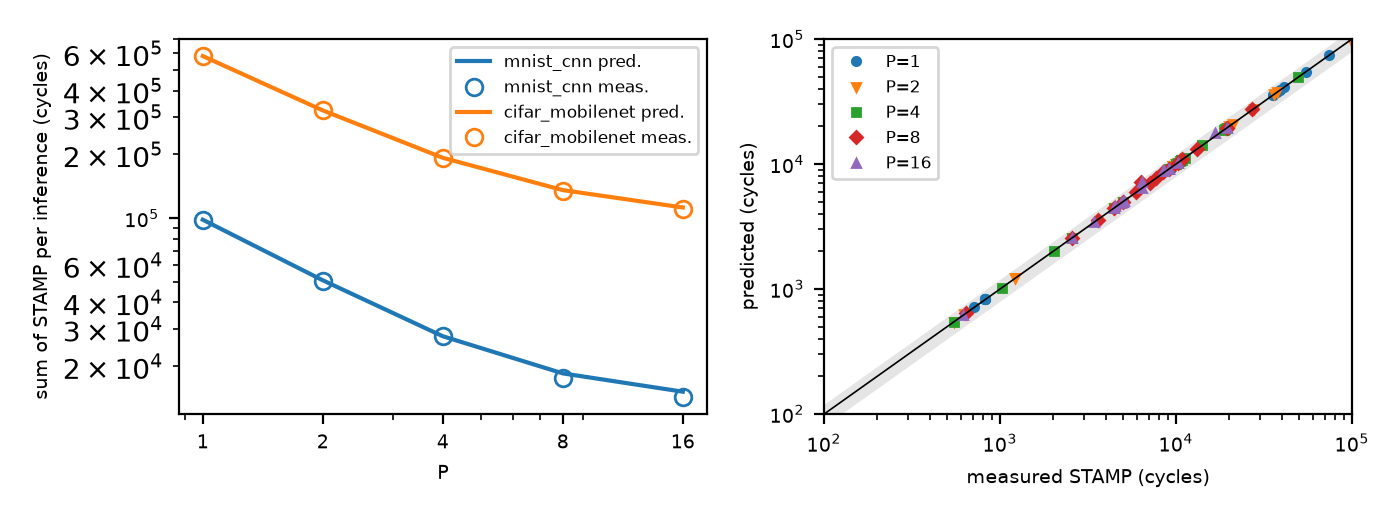
\includegraphics[width=0.8\textwidth]{m6_pred_vs_meas.png}
\caption{Frozen prediction (tag \texttt{m1}, \texttt{os} architecture) against measurement. Left: summed STAMP per inference versus $P$ (line: prediction, circles: measurement). Right: every scored command, predicted versus measured cycles; the band is $\pm\ThreshFourA\,\%$.}\label{fig:p}
\end{figure*}

\begin{table}[t]\centering\caption{Per-command cycles at $P=\PDefault$ (pred.\ from tag \texttt{m1}; meas.\ = median STAMP over the timed images).}\label{tab:cmd}
\footnotesize
% generated by experiments/make_macros.py from results/m1_predictions.csv (tag m1); do not edit
\tabtodo\begin{tabular}{llllrr}\toprule
net & op & kind & K & pred. & meas.\\\midrule
mnist & 1 & conv & 3x3 & 7,144 & 6,356 \\
mnist & 3 & conv & 3x3 & 7,756 & 7,715 \\
mnist & 7 & fc & 1x1 & 3,596 & 3,594 \\
cifar & 0 & conv & 3x3 & 27,724 & 27,029 \\
cifar & 1 & dw & 3x3 & 10,236 & 10,203 \\
cifar & 2 & conv & 1x1 & 8,712 & 8,452 \\
cifar & 3 & dw & 3x3 & 19,436 & 19,376 \\
cifar & 4 & conv & 1x1 & 10,888 & 10,883 \\
cifar & 5 & dw & 3x3 & 5,012 & 4,995 \\
cifar & 6 & conv & 1x1 & 5,928 & 5,923 \\
cifar & 7 & dw & 3x3 & 9,204 & 9,176 \\
cifar & 8 & conv & 1x1 & 10,536 & 10,469 \\
cifar & 9 & dw & 3x3 & 2,580 & 2,571 \\
cifar & 10 & conv & 1x1 & 7,096 & 7,077 \\
cifar & 11 & dw & 3x3 & 4,436 & 4,424 \\
cifar & 12 & conv & 1x1 & 13,240 & 13,237 \\
cifar & 15 & fc & 1x1 & 644 & 642 \\
\bottomrule
\end{tabular}

\end{table}

\section{Discussion and Limitations}
All cycle counts come from Verilator simulation; the FPGA is used only for synthesis figures (LUT, DSP, BRAM, Fmax). No FPGA wall-clock or power measurement exists yet; the procedure is in \texttt{HARDWARE\_TODO.md}, and wall-time speedup would be the cycle speedup scaled by the Fmax ratio of the SoC with and without the accelerator. The memory model is zero-wait on-chip RAM; an external memory would change the port-bound assumption. The accelerator covers convolution, depthwise (multiplier one) and fully connected layers only; pooling and layout ops stay in software and cap MNIST by Amdahl's law. The model has biases documented before \texttt{m1}, for example one extra setup cycle per pixel where a layer is requantizer bound; the setup bias proved larger than documented where the port and requantizer terms tie (above). Only two networks are evaluated. The repository has no remote, so the \texttt{m1} hash has not been timestamped externally; this is a manual step.

\section{Conclusion}
We built a small int8 accelerator and its backend and score an analytic model that was frozen before the RTL. The outcomes of the pre-registered claims are those in the tables above; they update from \texttt{results/} through \texttt{experiments/make\_macros.py}.

\section*{Acknowledgment}
AI assistance (Anthropic's Claude) was used to draft code and text; the authors take responsibility for all content.

\bibliographystyle{IEEEtran}
\bibliography{refs}
\end{document}
